
Notre étude porte sur trois groupes d'élèves de premières de lycée général suivant l'enseignement de spécialité NSI.
Deux groupes sont au lycée Monte-Cristo d'Allauch. Chaque groupe est composé de 18 élèves (dont 1 fille et un élève sourd pour l'un et 2 filles pour l'autre).
Le troisième groupe est au lycée Simone Veil de Marseille. Il est composé de 14 élèves (dont 2 filles).

La principale difficulté de notre étude porte sur le fait que nous ne pouvons pas anticiper les retards et/ou absences des élèves sur notre séance Jigsaw, car la constitution des groupes de niveaux est à faire en amont de la séance. Ainsi, nous nous devons de prévenir les élèves que nous allons effectuer une séance particulière, et ils se mettent donc peut-être une pression supplémentaire sur cette séance extraordinaire, ce qui peut biaiser notre étude.

Pour quantifier une pédagogie différenciée collaborative, nous proposons de travailler de la façon suivante :
\begin{enumerate}
	\item enseigner une même partie du programme de deux manières différentes en fonction des groupes :
	\begin{itemize}
		\item 1 ou 2 groupes témoins : méthode classique (cours magistral, TD, TP, évaluation).
		\item 1 ou 2 groupes tests : méthode Jigsaw.
	\end{itemize}
	\item évaluation sommative sur les notions abordées (recueil de performances académiques).
	\item évaluer un mois plus tard chacun des groupes avec un même support pour chaque groupe.
	\item reproduire ces premiers points sur une autre partie du programme en inversant les groupes test et témoin.
\end{enumerate}

Les variables de notre étude sont donc principalement quantitatives. En parallèle de celles-ci, nous avons décidé de filmer les séances afin d'obtenir des données plus qualitatives (à revoir $\rightarrow$ va-t-on analyser qualitativement ?)

Tableau qui guide la logique de la recherche, ne pas le recopier dans le mémoire.

\begin{center}
\begin{tabular}{|c|c|c|c|c|}
	\hline
	& \multicolumn{2}{|c|}{Variable 1 (Jigsaw)} & \multicolumn{2}{|c|}{Variable 2 (Pas Jigsaw)}\\
	\hline
	& Qualitative & Quantitative & Qualitative & Quantitative\\
	\hline
	Performance &  & x &  & x\\
	\hline
	Tutorat entre pairs & x &  & x & \\
	\hline
	Sollicitation enseignant & x &  & x & \\
	\hline
	Engagement activité & x &  & x & \\
	\hline
\end{tabular}
\end{center}

\begin{figure}[h!]
	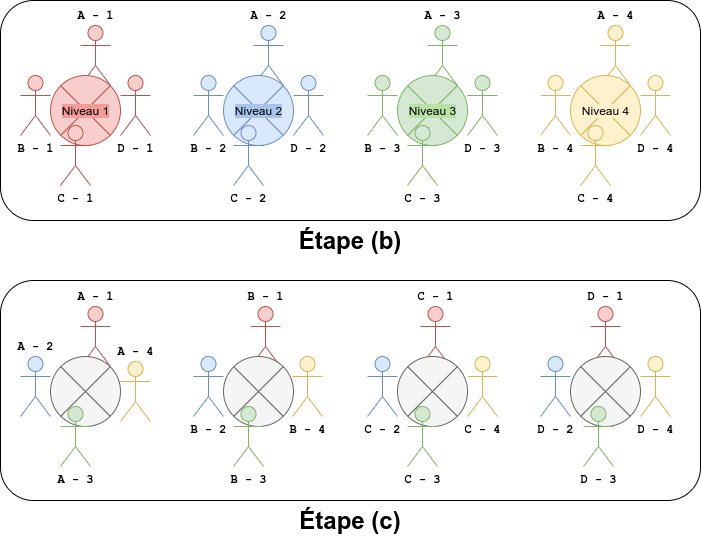
\includegraphics[width=\textwidth]{res/diagramme.drawio}
	\caption{Représentation de notre pédagogie collaborative}\label{SchémaNotreJigsaw}
\end{figure}

Nous avons choisi de travailler sur les deux notions suivantes provenant du programme officiel de première \gls{nsi} :
\begin{itemize}
	\item \emph{Représentation des données : types et valeurs de base} au sein de laquelle se trouvent les contenus suivants :
	\begin{description}
	    \item[Contenu 1] Écriture d'un entier positif dans une base $b=2$,
	    \item[Contenu 2] Écriture d'un entier positif dans une base $b>2$,
	    \item[Contenu 3] Représentation binaire d'un entier relatif,
	    \item[Contenu 4] Représentation approximative des nombres réels : notion de nombre flottant,
	    \item[Contenu 5] Valeurs booléennes, opérateurs booléens et expressions booléennes,
	    \item[Contenu 6] Représentation d'un texte en machine.
	\end{description}
	Nous avons choisi de retirer de notre étude les contenus 4 et 5 sur les notions booléennes, pour réduire le nombre de notions abordées lors de la séance Jigsaw et car nous avons considéré que ces notions peuvent être abordées dans une autre séquence.
	\item \emph{Constructions élémentaires des langages de programmation} au sein de laquelle se trouvent les contenus suivants :
	\begin{description}
	    \item[Contenu 1] Séquences d'instructions, variables et affectations,
	    \item[Contenu 2] Structures conditionnelles,
	    \item[Contenu 3] Structures itératives bornées,
	    \item[Contenu 4] Structures itératives non bornées,
	    \item[Contenu 5] Appels de fonction.
	\end{description}
	Nous avons choisi de retirer de notre étude le contenu 5 sur les appels de fonction, pour les mêmes raisons que précédemment.
\end{itemize}

\idee{Les contenus de programme étudiés lors des trois moments didactiques de notre méthodologie.}
Conformément à notre méthodologie, la séquence est partagée en trois moments didactiques distincts : le moment de la différenciation, le moment de l'appropriation et le moment de l'échange. 

Chacun de ces moments est l'occasion pour l'élève d'aborder les contenus de programme identifiés :

\begin{description}
    \item[Moment de la différenciation] qui permet à l'enseignant de créer trois groupes de niveau et à l'élève de (re)travailler les prérequis nécessaires lors des moments suivants :
    \begin{itemize}
        \item Contenu 1
    \end{itemize}
    \item[Moment de l'appropriation] qui permet à l'élève d'aborder un contenu adapté à son niveau parmi les trois possibles :
    \begin{itemize}
        \item Contenu 2 (pour un élève du groupe 1, niveau facile)
        \item Contenu 3 (pour un élève du groupe 2, niveau intermédiaire)
        \item Contenu 6 pour les types et valeurs de base, 4 pour les constructions élémentaires (pour un élève du groupe 3, niveau difficile)
    \end{itemize}
    \item[Moment de l'échange] qui permet à l'élève d'aborder les deux contenus du moment précédent qu'il n'a pas encore rencontré.
\end{description}

\idee{Des activités pour différencier les élèves.} 
L'objectif du moment de la différenciation est de créer des groupes de niveaux. L'intérêt de cette discrimination des élèves est de proposer lors du moment de l'appropriation un travail adapté au niveau de chacun.
\info{\#TODO ajouter une source théorique}
Ainsi à l'issue de notre séance chaque élève, quel que soit son niveau, aura été à fois récepteur mais aussi et surtout transmetteur de savoir-faire auprès de son groupe d'échange.

Pour différencier les élèves, nous utilisons des activités qui sont construites pour être réalisées par les élèves en autonomie. Ces activités nous permettent d'établir un diagnostic concernant l'aisance des élèves sur le contenu 1.

\idee{Décomposition des contenus du programme en tâches pour décrire le travail de l'élève}
Afin de mieux décrire le travail de l'élève à l'issue de ces activités, nous proposons une décomposition en tâches des contenus du programme abordées lors du moment de la différenciation. Cette décomposition en tâches permet donc de clarifier l'objectif de chacune des activités du moment de la différenciation.
